\hfill \smallbreak
Tinc je još jedan besplatan program za uspostavu VPN veze. Ono po čemu se tinc razlikuje od drugih programa je niz jedinstvenih mogućnosti koje uključuje, kao što su enkripcija, neobavezna kompresija, automatsko usmjeravanje u mreži „svatko sa svakim“, lagano proširivanje… Ove mogućnosti čine tinc jako dobrim rješenjem za poslovne mreže koje su sastavljene od velikog broja manjih udaljenih mreža. Slijede upute za instalaciju, konfiguraciju i pokretanje tinc-a.

\subparagraph{Instalacija}
\hfill \smallbreak
Prvo preuzmemo instalacijski paket s adrese 
\url{http://www.tinc-vpn.org/packages/windows/tinc-1.1pre15-install.exe} te obavimo standardi instalacijski postupak, pokrenemo installer, next, prihvatimo uvjete korištenja, Ok, označimo sva polja kada nas pita koje komponente želimo instalirati, next, install, finish. \\Slijedi postupak za postavljanje računala poslužitelja, ovaj postupak radimo na računalu koje se nalazi u mreži kojoj želimo pristupati koristeći udaljeno računalo klijent. Otvorimo mapu u koju smo instalirali tinc (vjerojatno C:\textbackslash Program Files\textbackslash tinc) unutar komandne linije koju smo pokrenuli kao administrator, pozicioniramo se u mapu C:\textbackslash Program Files\textbackslash tinc te upisujemo redom naredbe (u zagradama se nalaze komentari, njih ne upisujemo u komandnu liniju):
\FloatBarrier
\smallbreak \code{tinc -n vpn init master}
\smallbreak \code{tinc -n vpn add subnet 20.0.1.1} (dodjela ip-adrese koju želimo da ima, na primjer 20.0.1.1)
\smallbreak \code{tinc -n vpn add address=FQDNORIP}  (gdje je FQDNORIP javna IP adresa poslužiteljskog računala)
\smallbreak \code{cd tap-win64}
\smallbreak \code{addtap.bat}
\smallbreak \code{cd ..}
\smallbreak \code{netsh interface ipv4 show interfaces}  (pogledamo što je odspojeno, vjerojatno Ethernet 2)
\smallbreak \code{netsh interface set interface name = "Ethernet 2" newname = "tinc"}
\smallbreak \code{netsh interface ip set address "tinc" static 20.0.1.1    255.255.255.0}
\smallbreak \code{netsh interface ipv4 show config}  (sada bi trebali imati sučelje „tinc“ s maskom podmreže i IP-adresom)\\
\FloatBarrier
Time je konfiguriran poslužitelj. Sada sličan postupak moramo ponoviti za računalo klijent. Na njemu također nakon instalacije pokrenemo komandnu liniju kao administrator i pozicioniramo se u mapu gdje je tinc instaliran te upišemo sljedeće naredbe:
\FloatBarrier
\smallbreak \code{tinc -n vpn init client1}
\smallbreak \code{tinc -n vpn add connectto master}
\smallbreak \code{tinc -n vpn add subnet 20.0.2.2}
\smallbreak \code{cd tap-win64}
\smallbreak \code{addtap.bat}
\smallbreak \code{cd ..}
\smallbreak \code{netsh interface ipv4 show interfaces}  (pogledamo što je odspojeno, vjerojatno Ethernet 2)
\smallbreak \code{netsh interface set interface name = "Ethernet 2" newname = "tinc"}
\smallbreak \code{netsh interface ip set address "tinc" static 20.0.2.2 255.255.255.0}\\
\FloatBarrier
Potrebno je još samo s klijentskog računala kopirati datoteku vpn/hosts/client1 na poslužiteljsko računalo u mapu vpn/hosts
i s poslužiteljskog računala kopirati datoteku vpn/hosts/master na klijentsko računalo u mapu vpn/hosts. Sada je sve spremno za korištenje.

\subparagraph{Pokretanje}
\hfill \smallbreak
Kada je završena instalacija i konfiguracija, mreža će izgledati kao mreža sa slike 41., a tinc se pokrene jednostavnom naredbom koja je jednaka za klijenta i poslužitelja:
\FloatBarrier
\smallbreak \code{tincd -n vpn -D -d3}
\FloatBarrier
\begin{figure}[h!]
	\centering
     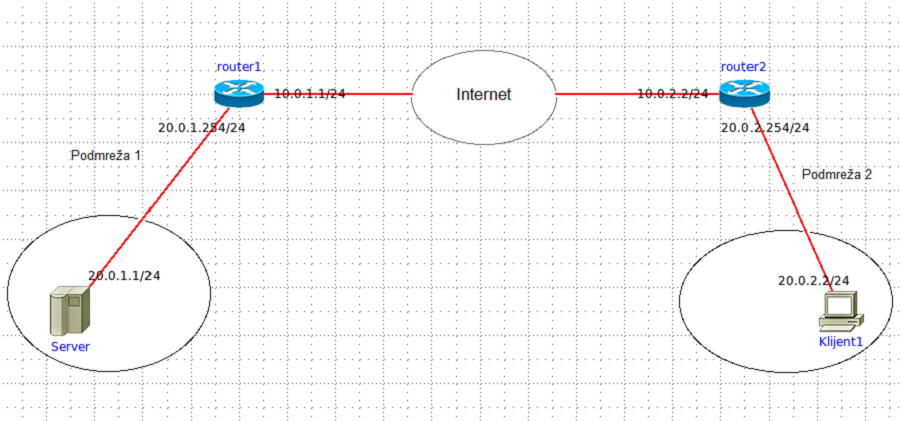
\includegraphics[width=0.8\textwidth]{Tinc/Slika41}
     \caption{Izgled mreže nakon uspostave VPN-a}
\end{figure}
\FloatBarrier